\section{Tests on the prototypes and results}
\subsection{Preliminary tests at IRMA}
\begin{frame}
  \frametitle{Test at IRMA}
  \begin{columns}
    \begin{column}{0.45\textwidth}
      Tests of silicon detector at IRMA:
      \begin{itemize}
        \item Ion implantation source
        \item $5$ to $190\,\mathrm{keV}$
        \item Many species
      \end{itemize}
      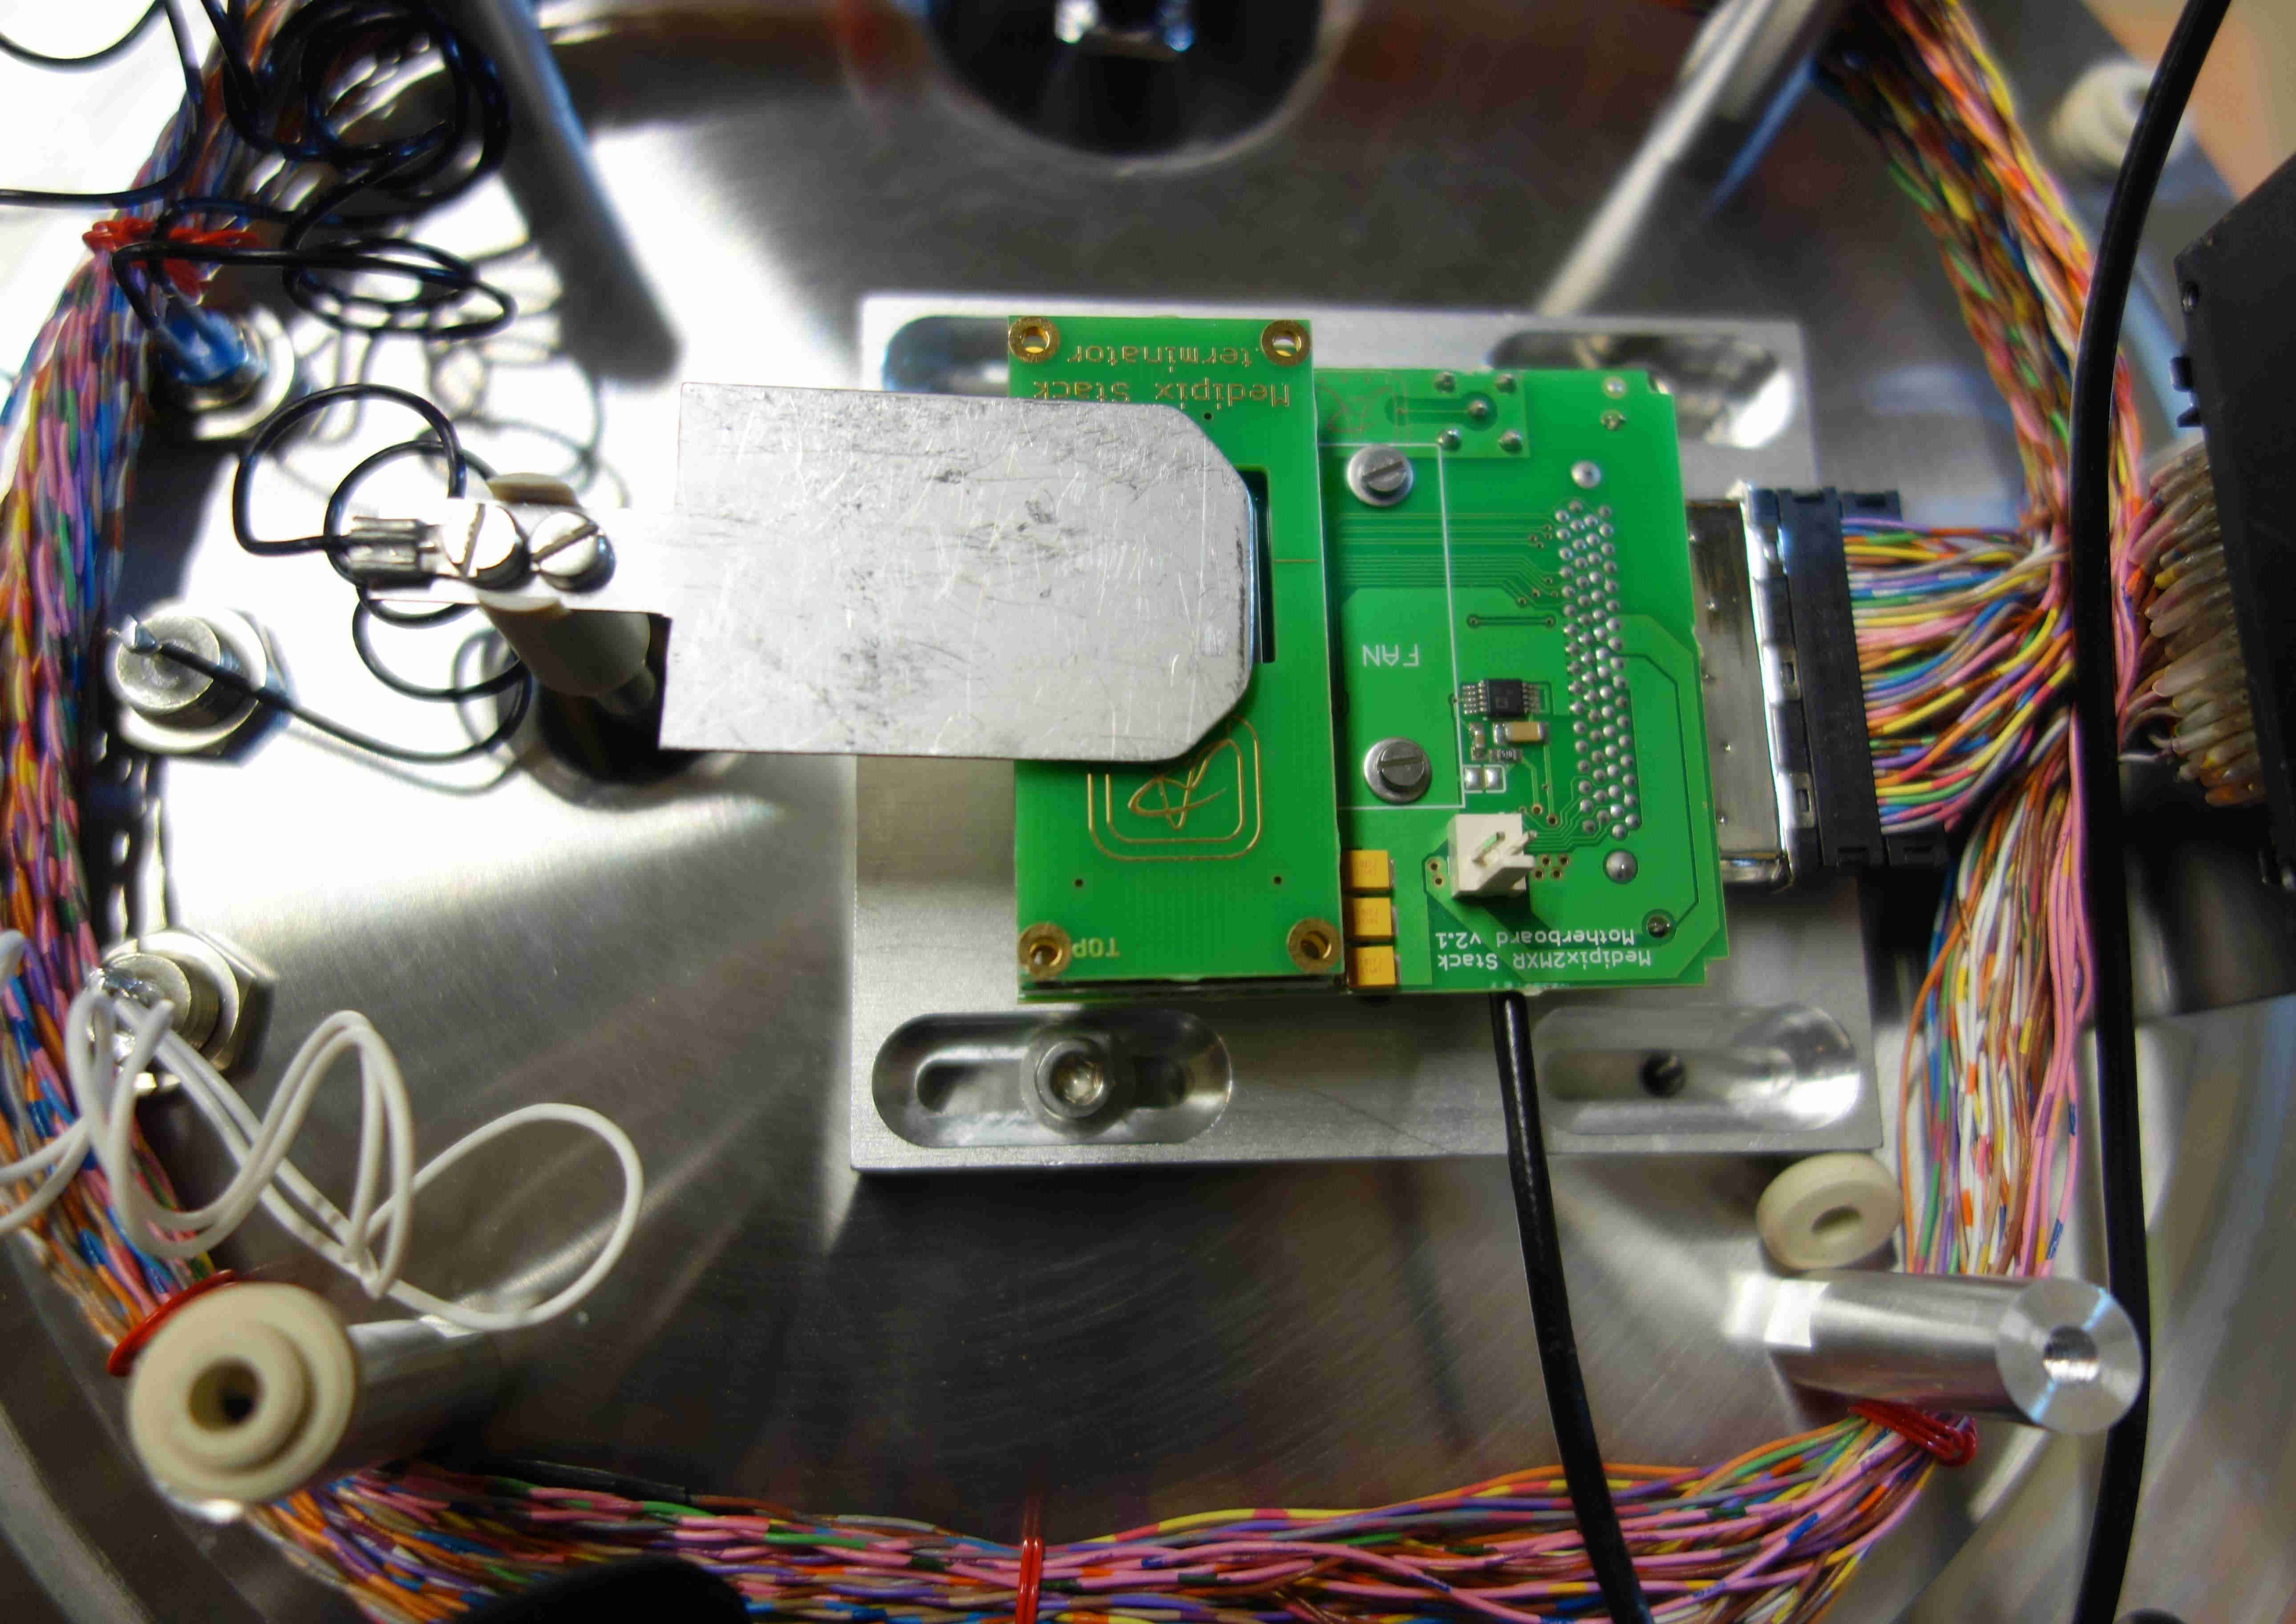
\includegraphics[width=\textwidth]{04_Test/fig/fig000_IRMA_setup01.jpg}
    \end{column}
    \begin{column}{0.45\textwidth}
      \begin{columns}
        \begin{column}{0.45\textwidth}
          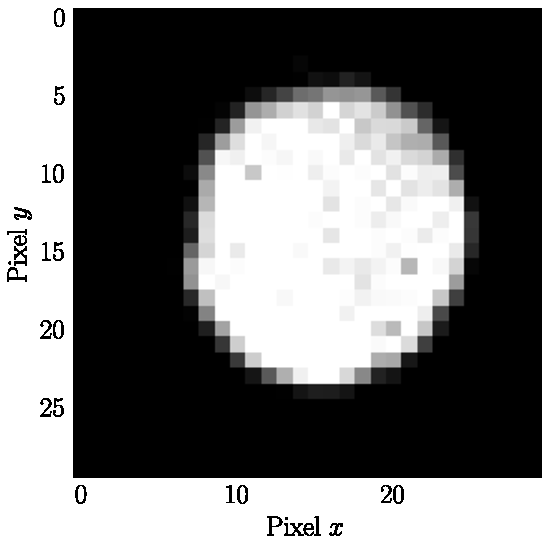
\includegraphics[width=\textwidth]{04_Test/fig/fig000_IRMA_15keV_svg-tex.pdf}
        \end{column}
        \begin{column}{0.45\textwidth}
          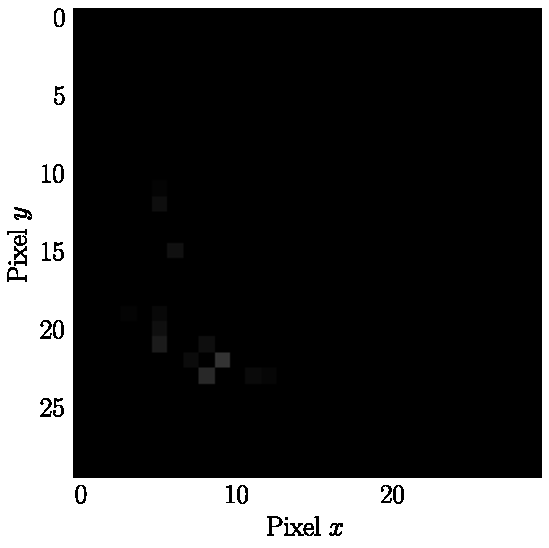
\includegraphics[width=\textwidth]{04_Test/fig/fig000_IRMA_12keV_svg-tex.pdf}
        \end{column}
      \end{columns}
      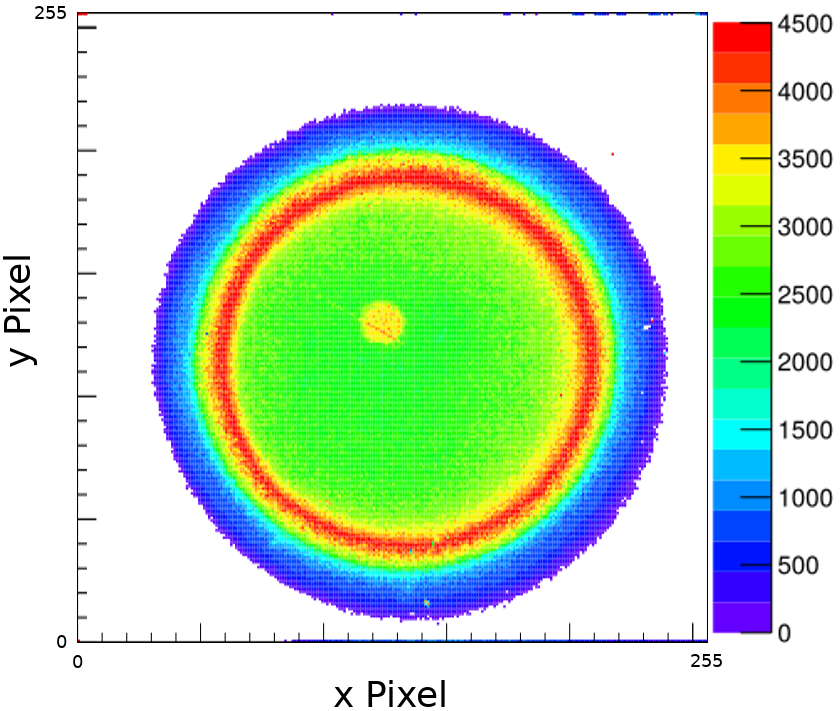
\includegraphics[width=\textwidth]{04_Test/fig/fig000_IRMA_damage3.png}
    \end{column}
  \end{columns}
  \begin{alertblock}{It works but too risky}
    We discarded the silicon/TimePix option.
  \end{alertblock}
\end{frame}

\subsection{IPM testbench}
\begin{frame}
  \frametitle{IPM prototype}
  \begin{columns}
    \begin{column}{0.45\textwidth}
      IPM prototypes have been built

      \begin{itemize}
        \item The cage is
        \item The readout can be easily changed.
      \end{itemize}

      \begin{itemize}
        \item Macor
        \item PEEK
        \item
      \end{itemize}

    \end{column}
    \begin{column}{0.45\textwidth}
      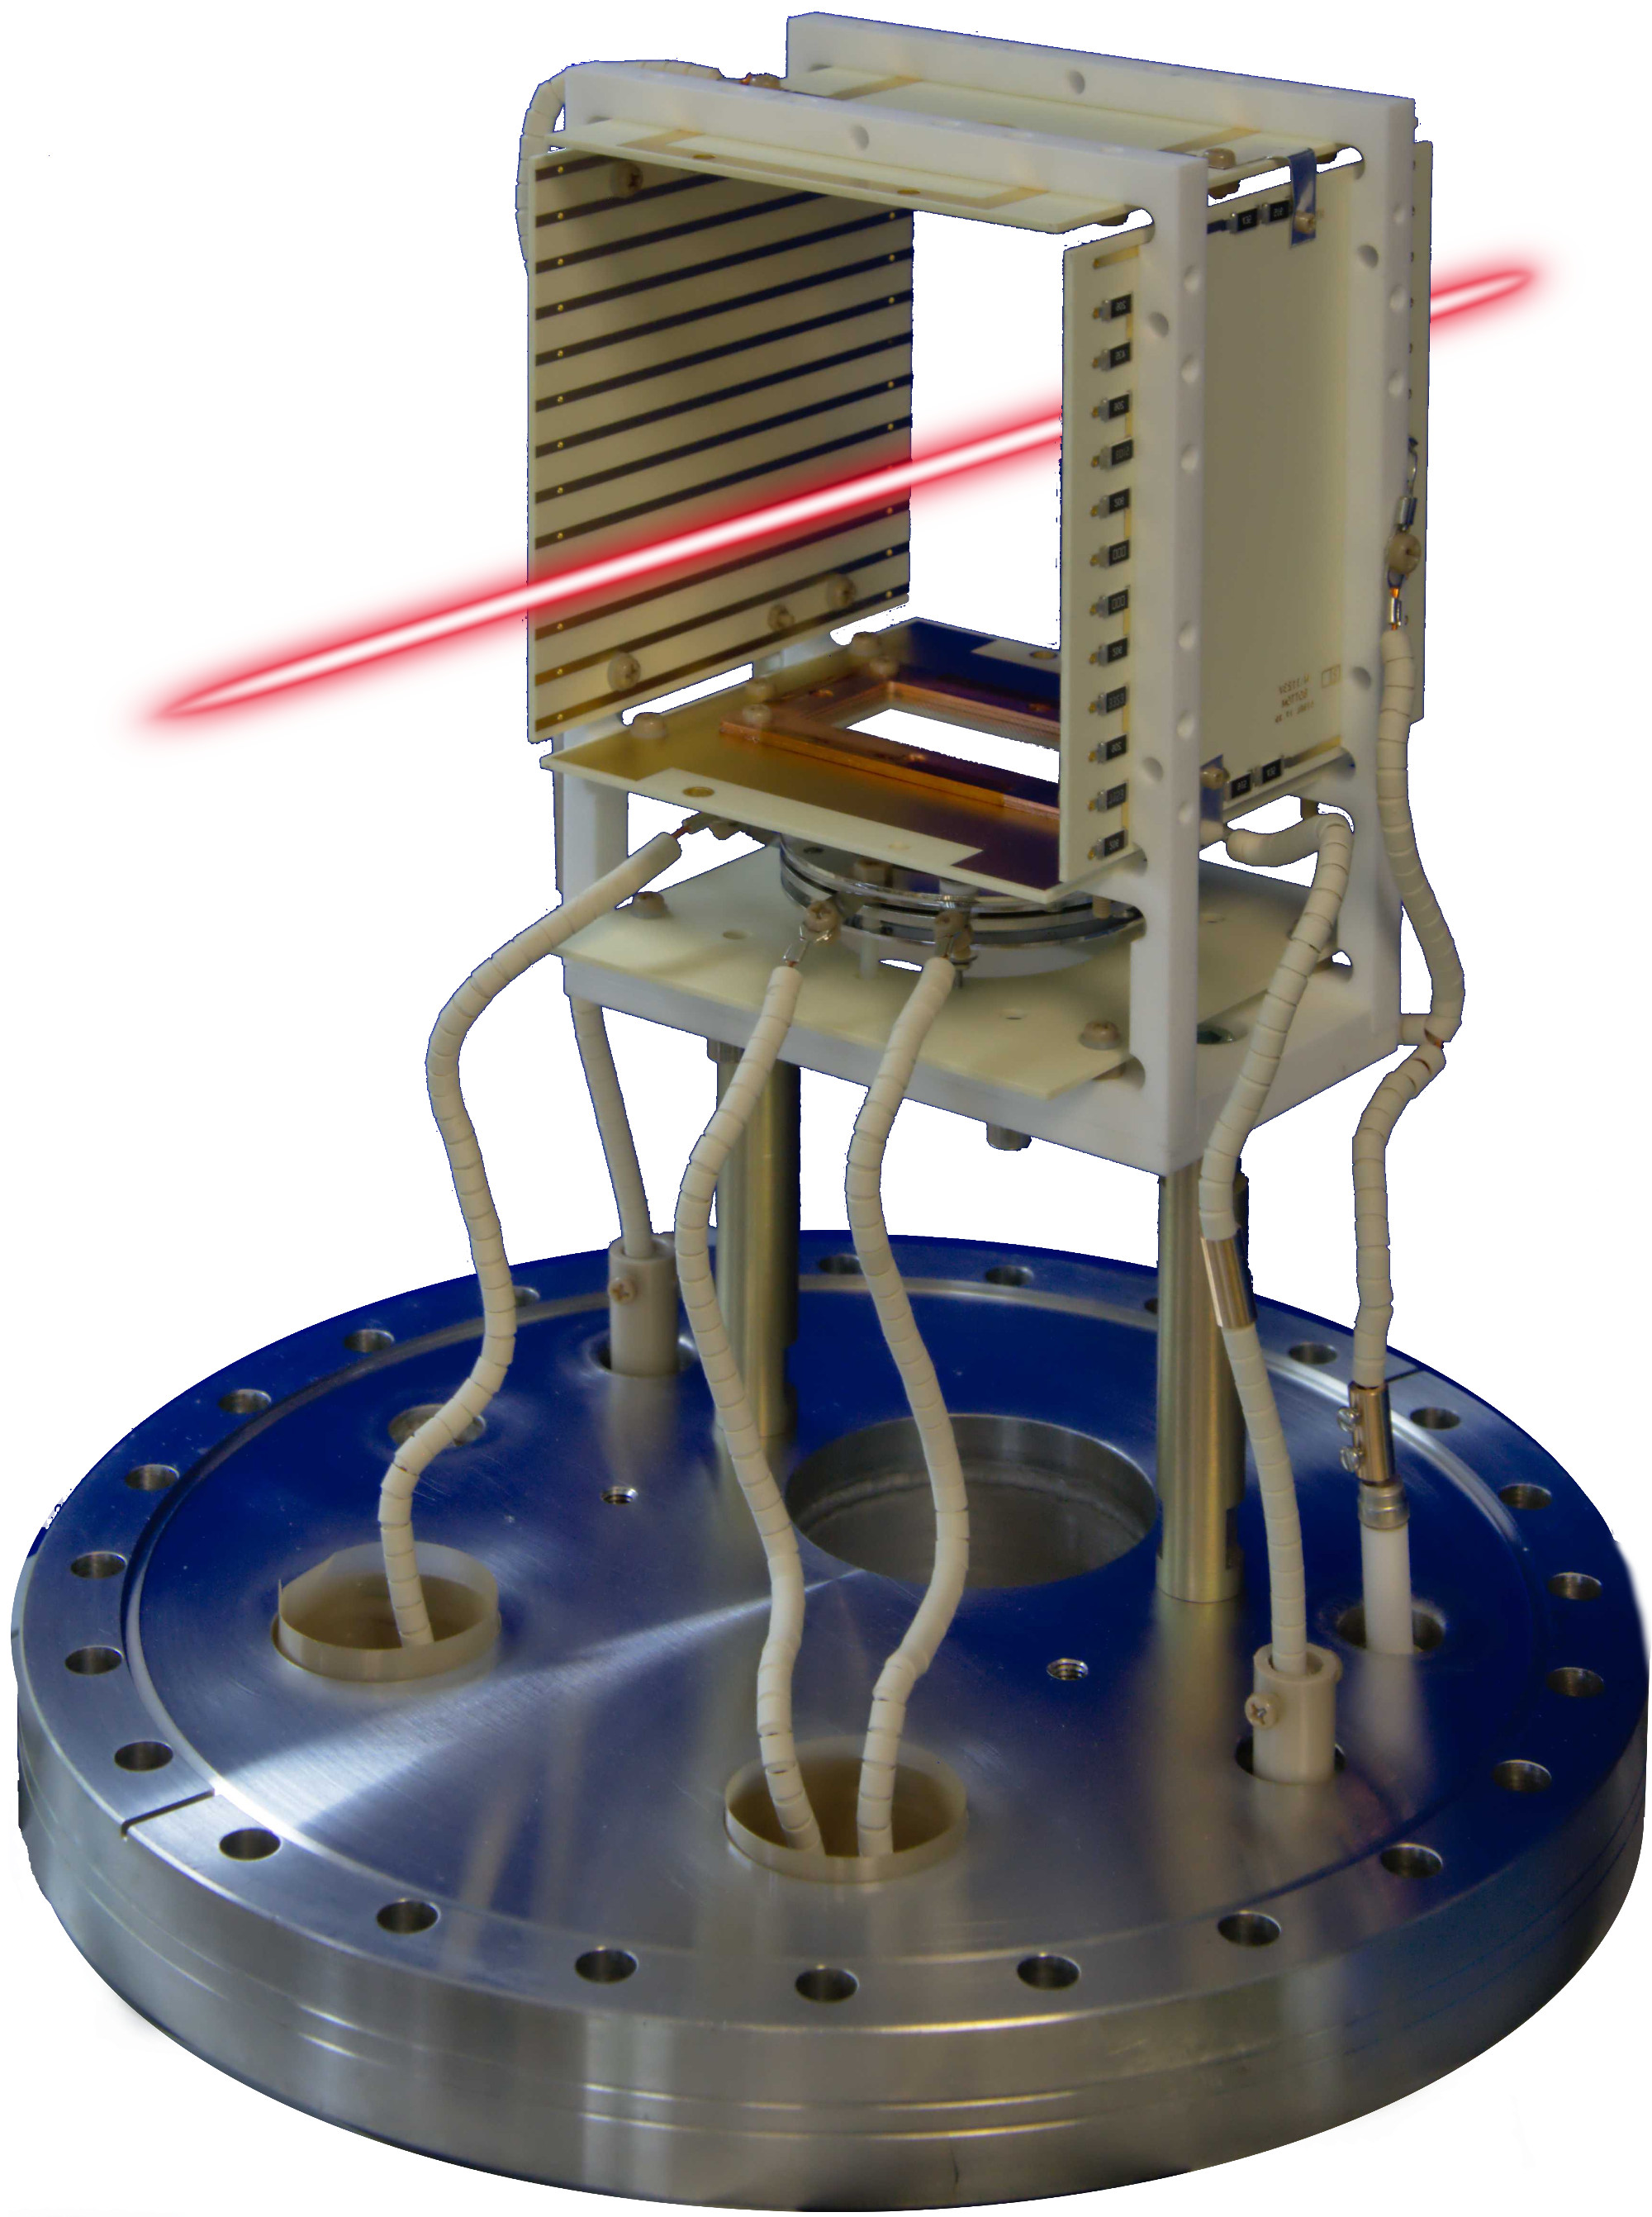
\includegraphics[width=\textwidth]{04_Test/fig/fig000_IPM_photo2}
    \end{column}
  \end{columns}
\end{frame}

\begin{frame}
  \frametitle{IPM test bench}
  As well, a dedicated test bench has been developed:
  \begin{center}
    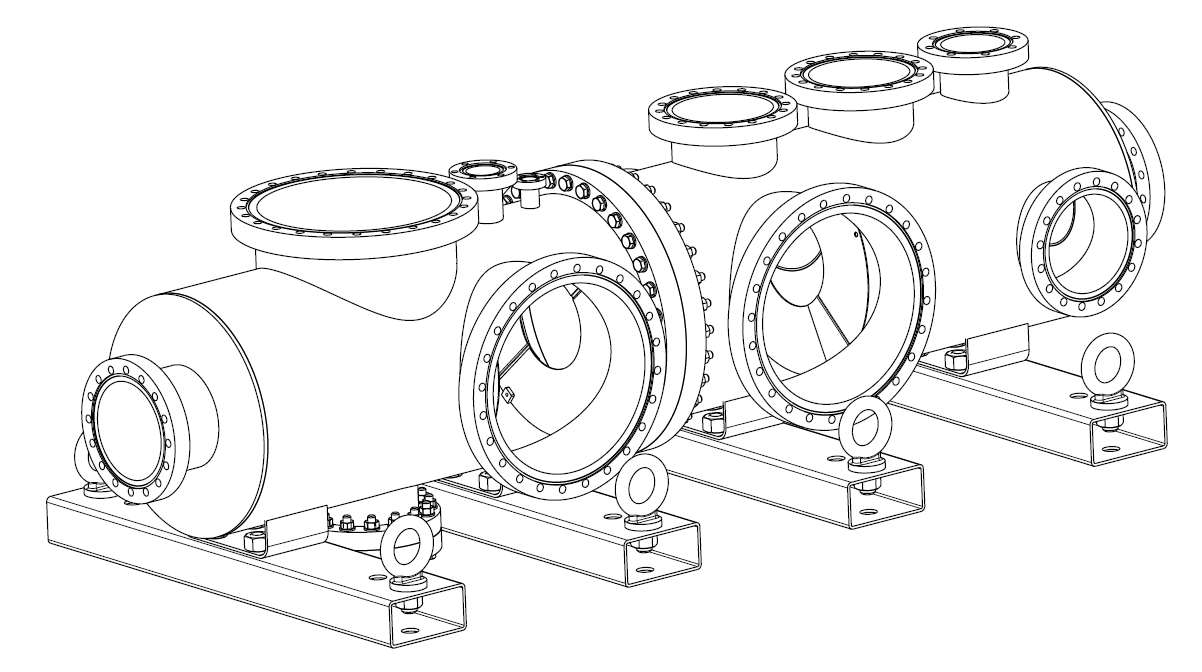
\includegraphics[width=0.7\textwidth]{04_Test/fig/fig000_Testbench.png}
  \end{center}
  \begin{columns}[T]
    \begin{column}{0.45\textwidth}
      \begin{block}{Upstream}
        \begin{itemize}
          \item Mimic ESS LWU geometry.
          \item 2 slot for IPM prototypes.
        \end{itemize}
      \end{block}
    \end{column}

    \begin{column}{0.45\textwidth}
      \begin{block}{Downstream}
        \begin{itemize}
          \item Extension adding more slots.
          \item 1 slot for an IPM prototype.
          \item 2 slot for reference measurements.
        \end{itemize}
      \end{block}
    \end{column}
  \end{columns}

\end{frame}

\subsection{IPHI}
\begin{frame}
  \frametitle{IPHI}
  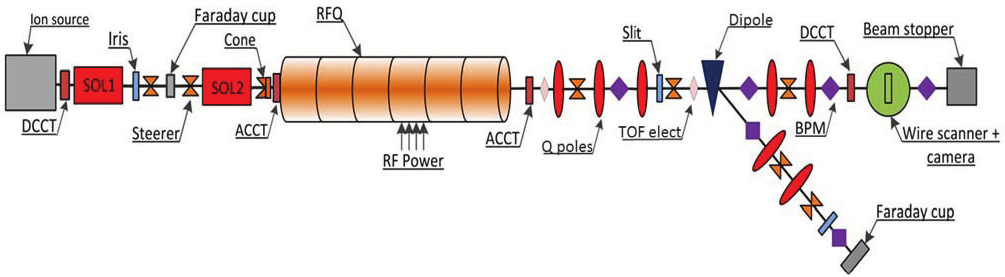
\includegraphics[width=1\textwidth]{04_Test/fig/fig000_IPHI_view.png}
  \begin{tabularx}{\linewidth}{XXX}
    \toprule
                         & IPHI accelerator                                  & ESS accelerator                \\
    \midrule
    Energy               & $3\,\mathrm{MeV}$                                 & $2\,\mathrm{GeV}$              \\
    Max current          & $0.5-100\,\mathrm{mA}$                            & $62.5\,\mathrm{mA}$            \\
    Max pulse duration   & $>100\,\mathrm{\mu s}$ up to DC                   & $2.86\,\mathrm{ms}$            \\
    Max pulse repetition & -                                                 & $14\,\mathrm{Hz}$              \\
    Vacuum range         & $5\cdot10^{-7}$ to $1\cdot10^{-8}\,\mathrm{mbar}$ & $1\cdot10^{-9}\,\mathrm{mbar}$ \\
    \bottomrule
  \end{tabularx}
  \begin{alertblock}{IPHI can be seen as the 20 first meter of ESS}
    Same , but lower energy $\implies$ more signal:
    \begin{itemize}
      \item dd
      \item In these conditions the beam may be
    \end{itemize}
  \end{alertblock}
\end{frame}

\begin{frame}
  \frametitle{IPHI test campaign}
  \begin{columns}[T]
    \begin{column}{0.45\textwidth}
      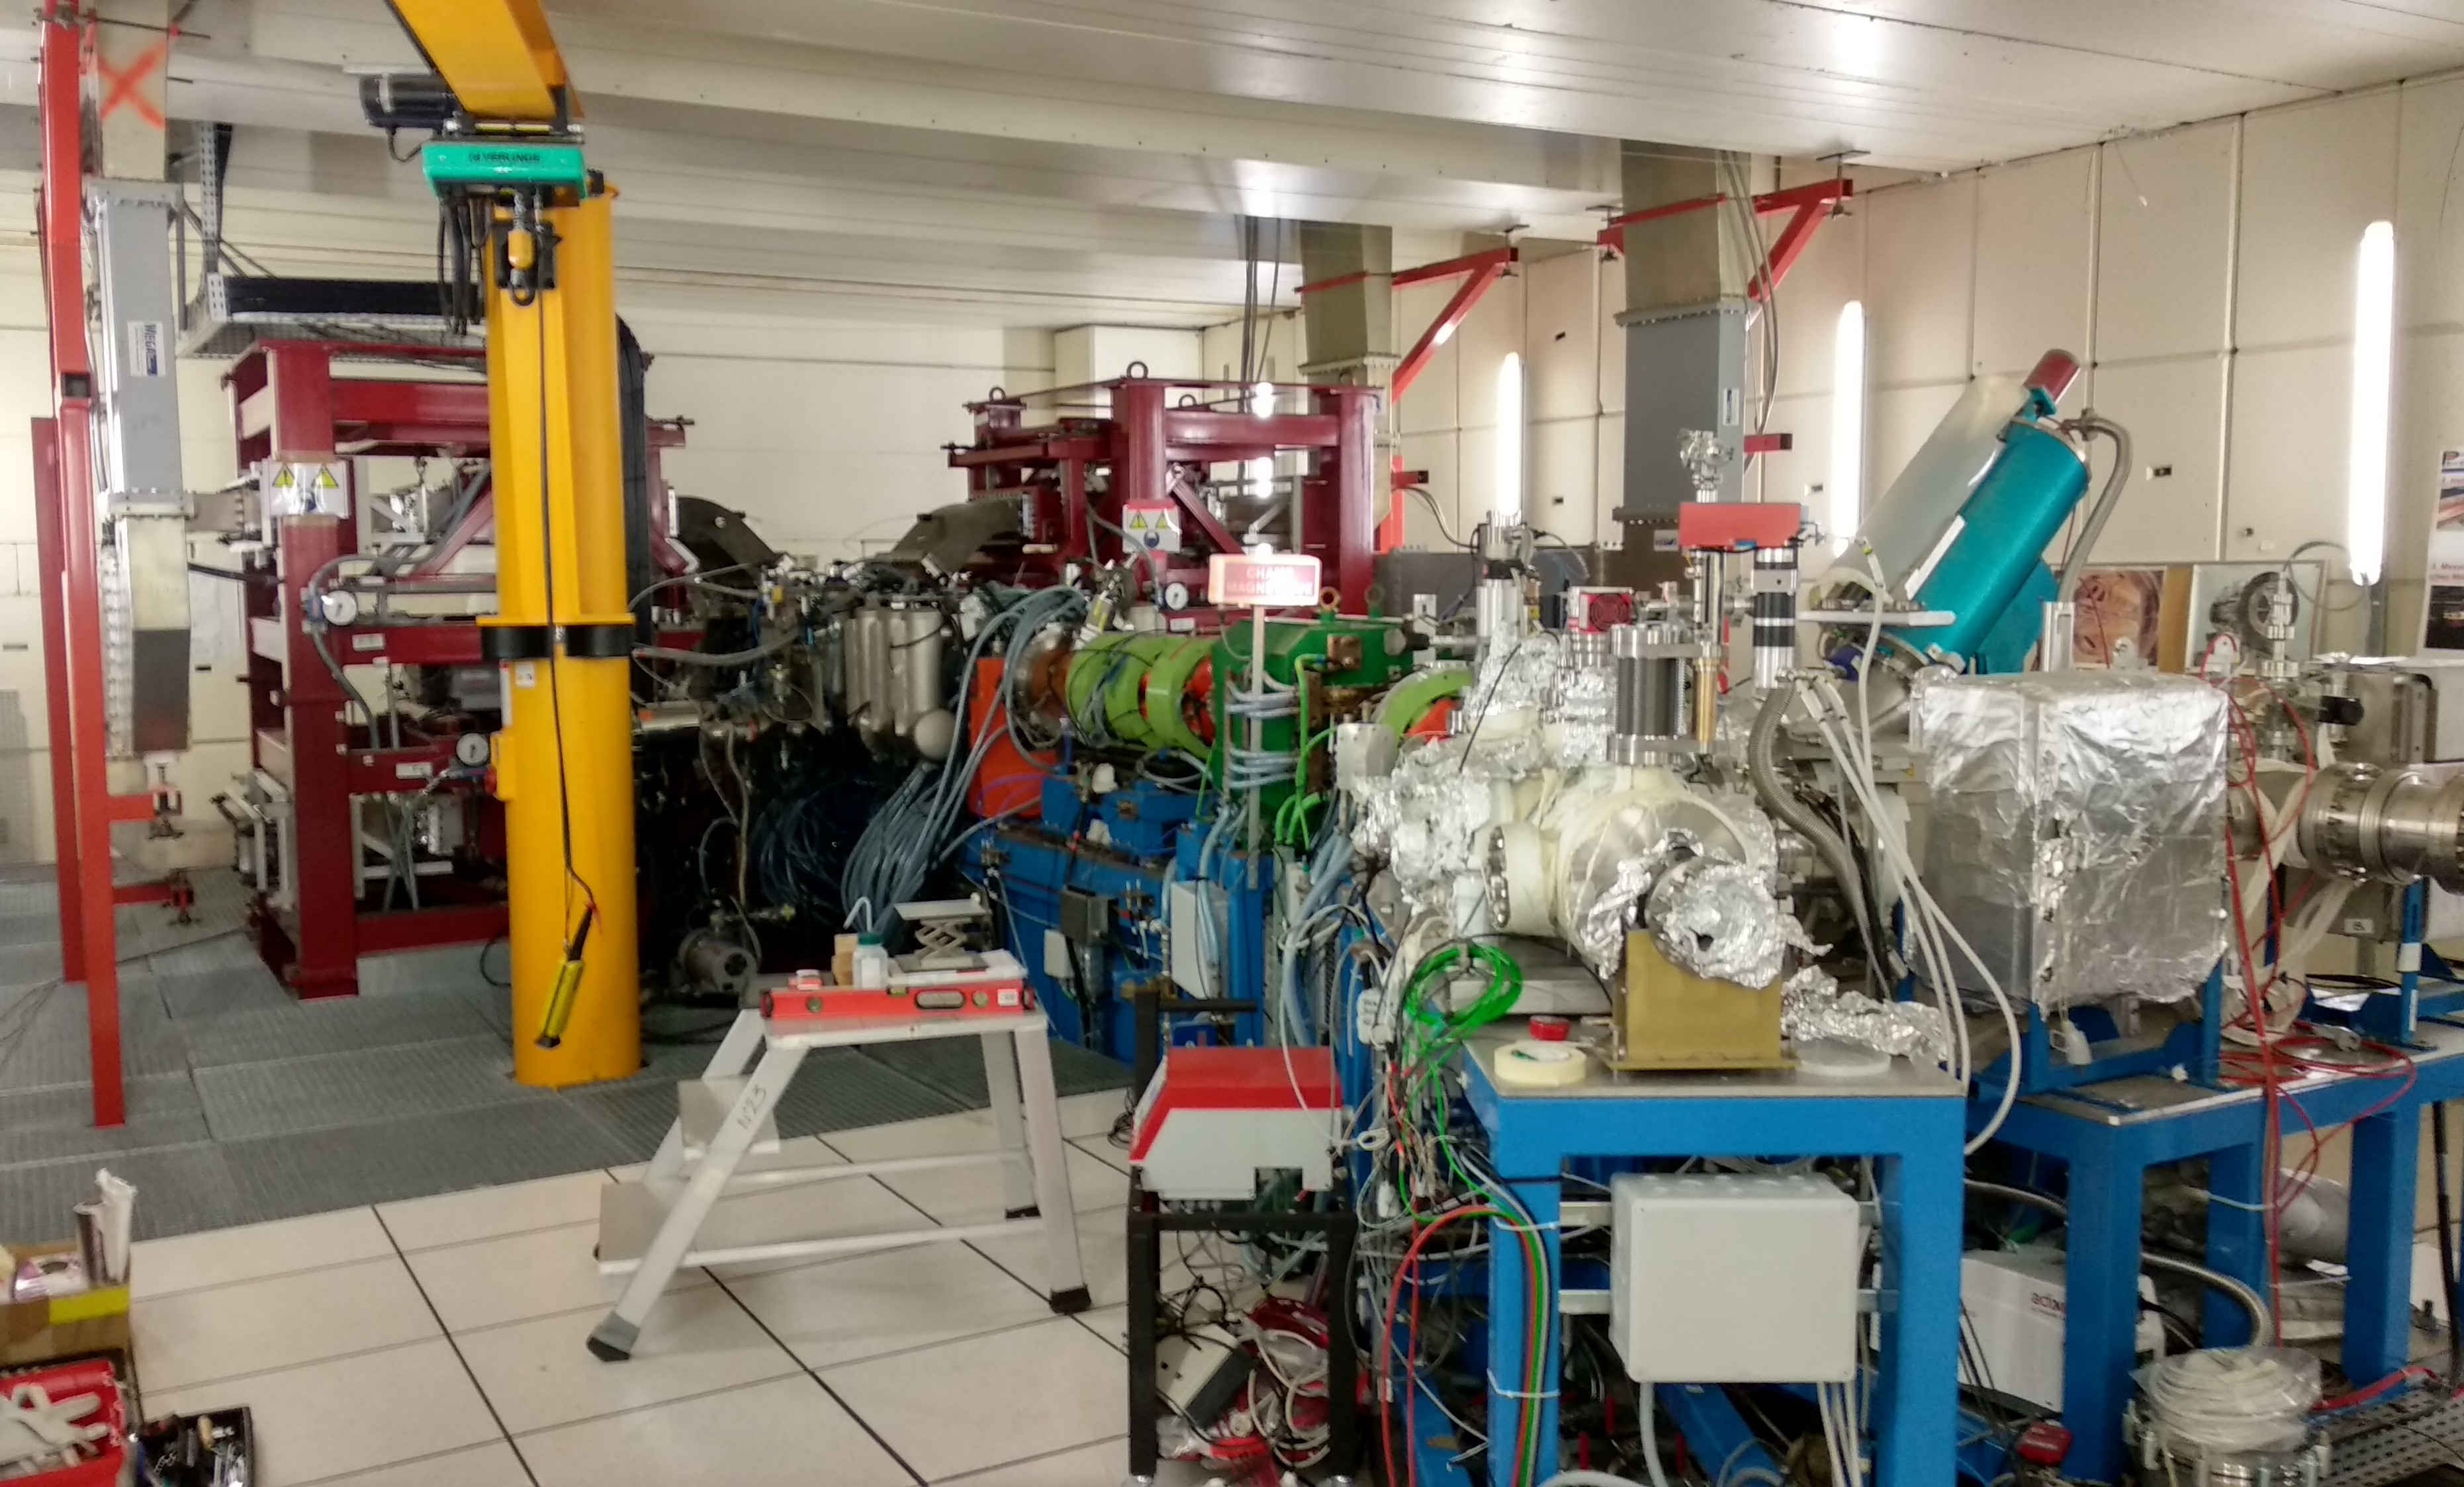
\includegraphics[width=1\textwidth]{04_Test/fig/fig000_IPHI_tb1.jpg}
    \end{column}
    \begin{column}{0.45\textwidth}
      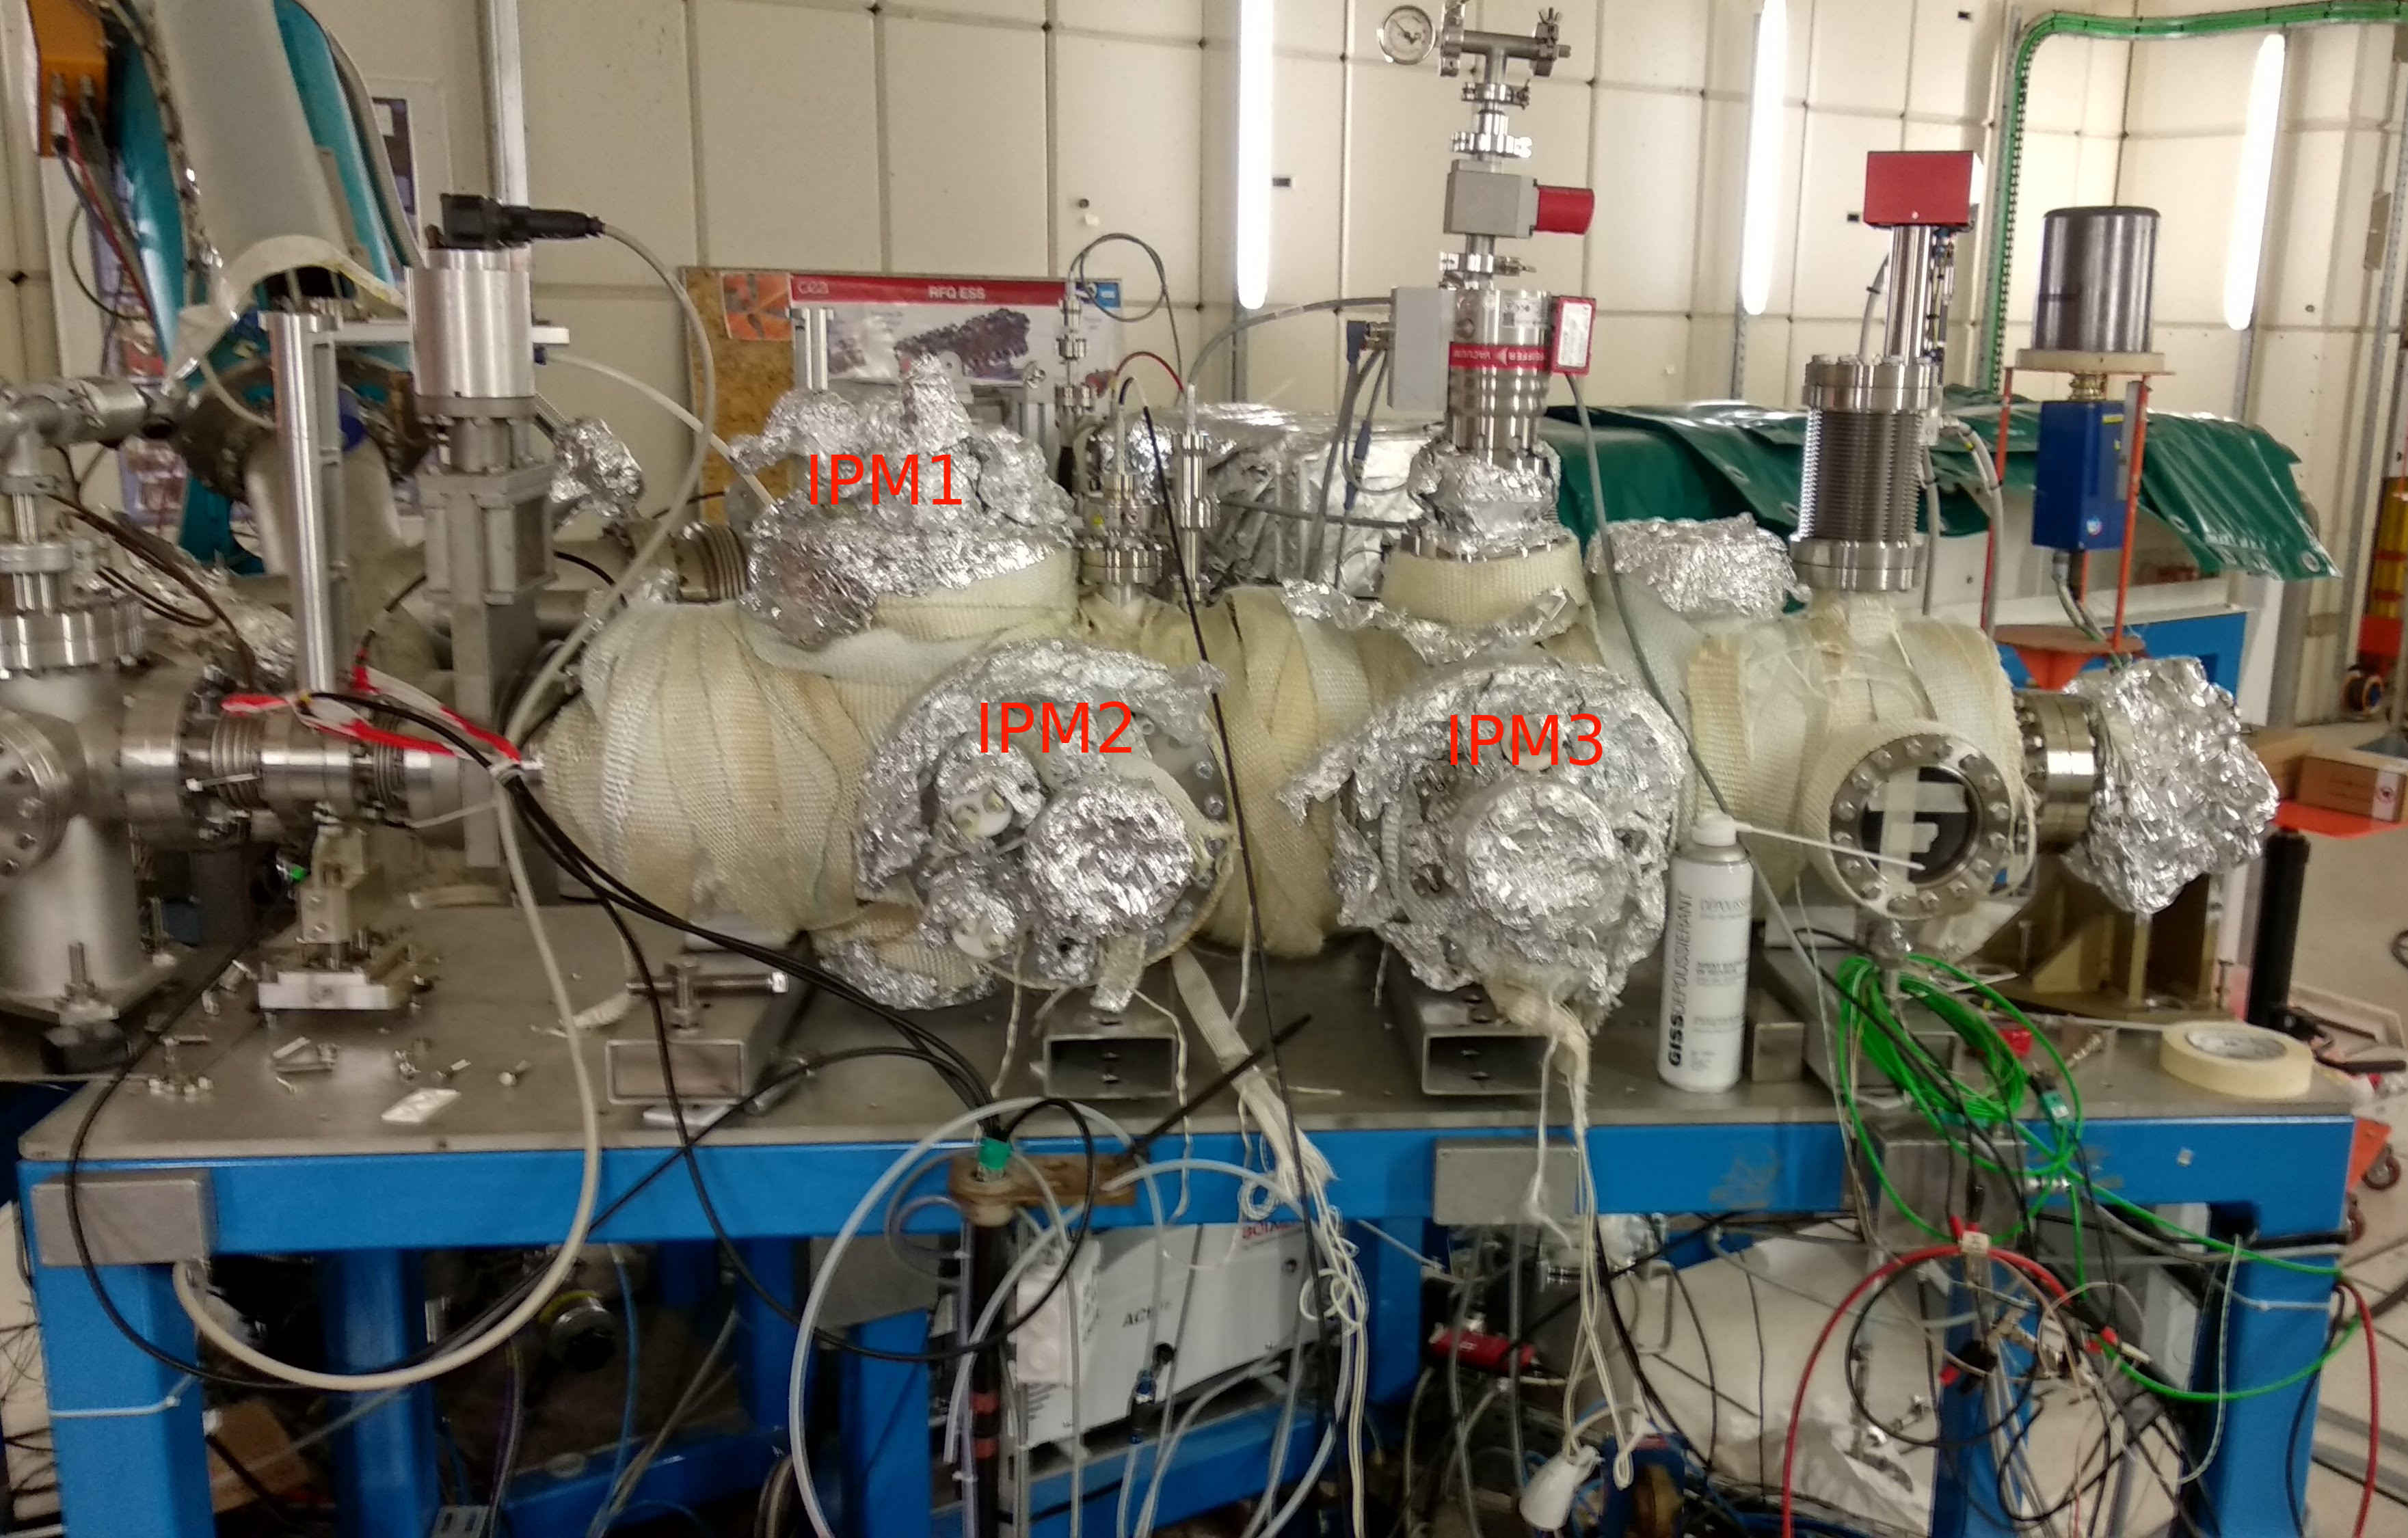
\includegraphics[width=1\textwidth]{04_Test/fig/fig000_IPHI_tb2.jpg}
    \end{column}
  \end{columns}
\end{frame}

\subsection{Results}
\begin{frame}
  \frametitle{Processing data}
  \begin{columns}[T]
    \begin{column}{0.45\textwidth}
      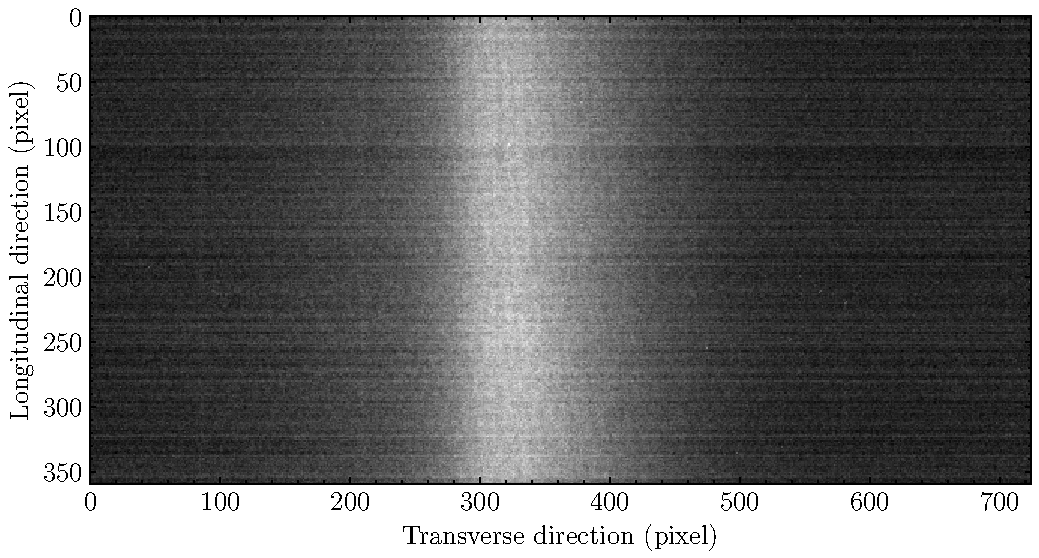
\includegraphics[width=1\textwidth]{04_Test/fig/fig000_image_beam}
    \end{column}
    \begin{column}{0.45\textwidth}
      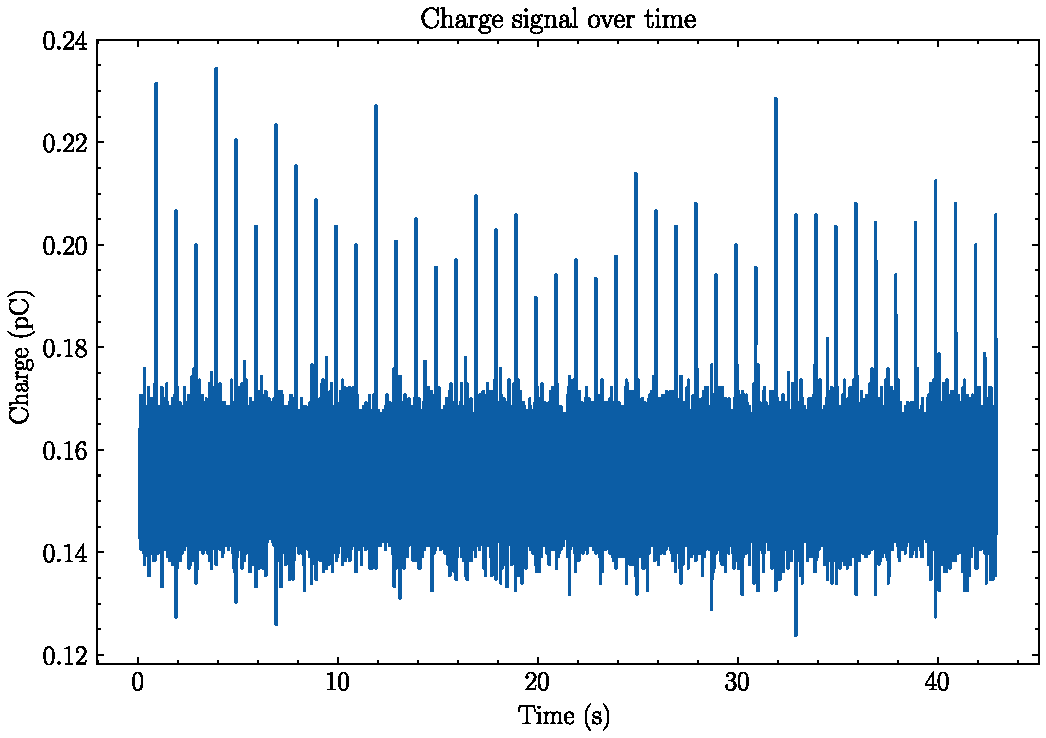
\includegraphics[width=1\textwidth]{04_Test/fig/fig000_strips_signal}
    \end{column}
  \end{columns}
  \begin{columns}[T]
    \begin{column}{0.45\textwidth}
      \begin{block}{Processing}
        \begin{enumerate}
          \item Crop image to ROI
          \item Remove dead pixel
          \item Filtering
          \item Sum along longitudinal direction
        \end{enumerate}
      \end{block}
    \end{column}
    \begin{column}{0.45\textwidth}
      \begin{block}{Processing}
        \begin{enumerate}
          \item Crop image to ROI
          \item Remove dead pixel
          \item Filtering
          \item Sum along longitudinal direction
        \end{enumerate}
      \end{block}
    \end{column}
  \end{columns}
\end{frame}

\begin{frame}
  \frametitle{Profile comparison between IPM}
  \begin{center}
    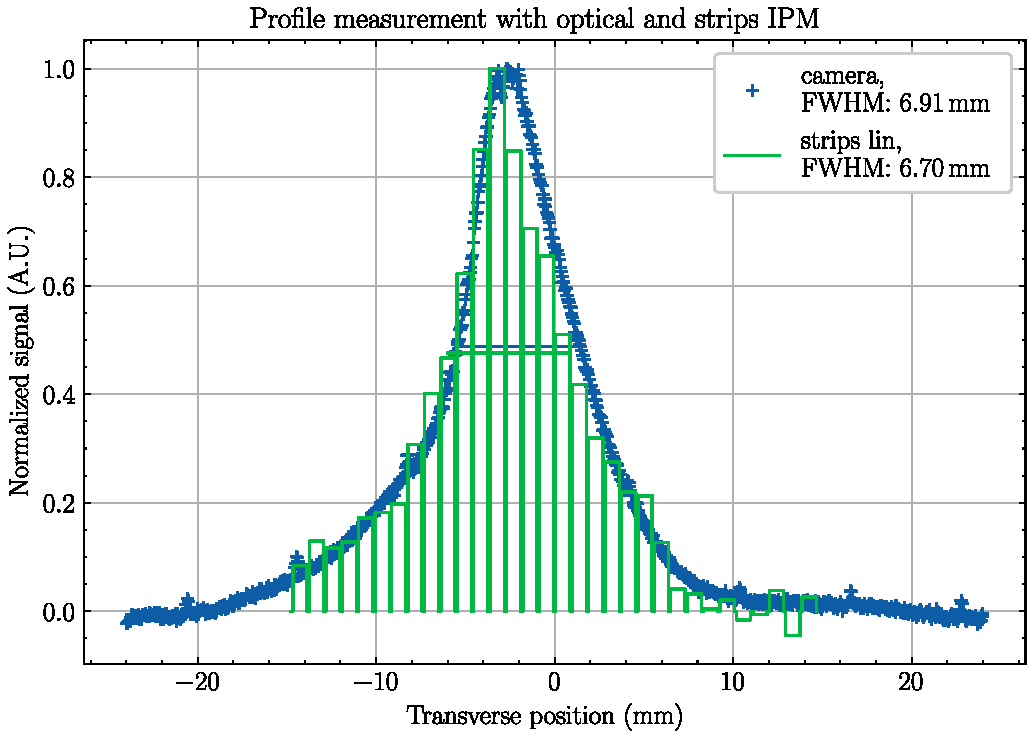
\includegraphics[width=0.75\textwidth]{04_Test/fig/fig000_MCP_strip}

  \end{center}
  \begin{block}{XX}
    XX
  \end{block}
\end{frame}

\begin{frame}
  \frametitle{Limitation}
  \begin{columns}[T]
    \begin{column}{0.45\textwidth}
      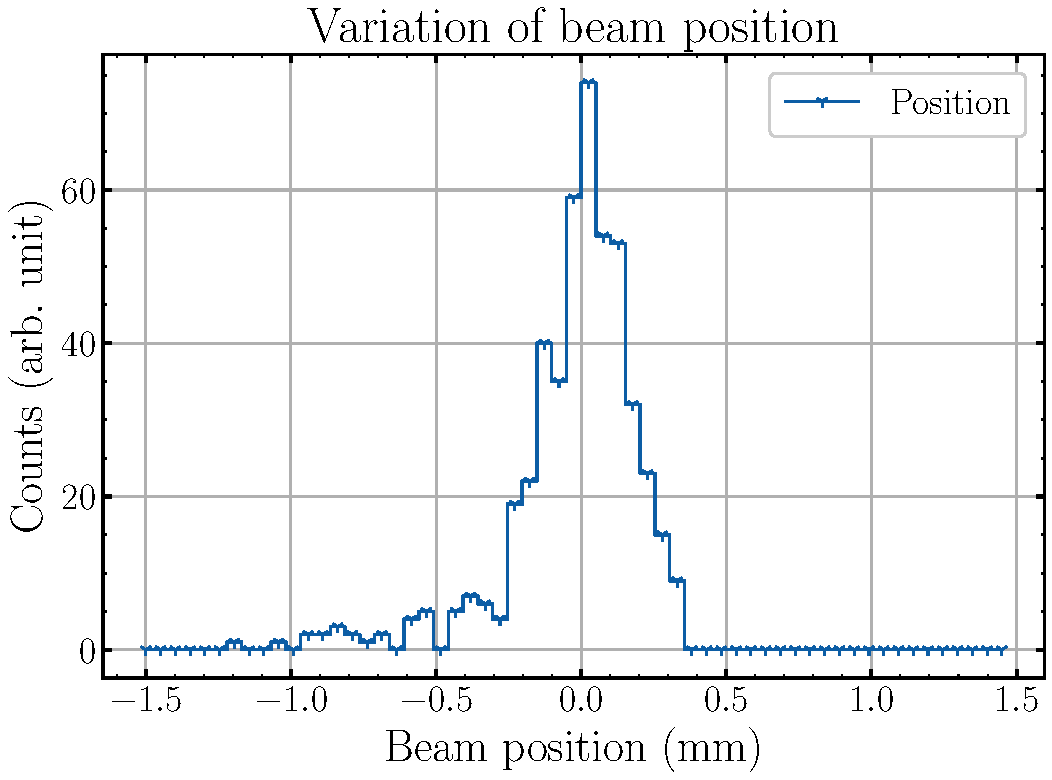
\includegraphics[width=1\textwidth]{04_Test/fig/fig000_hist_variation_a}
      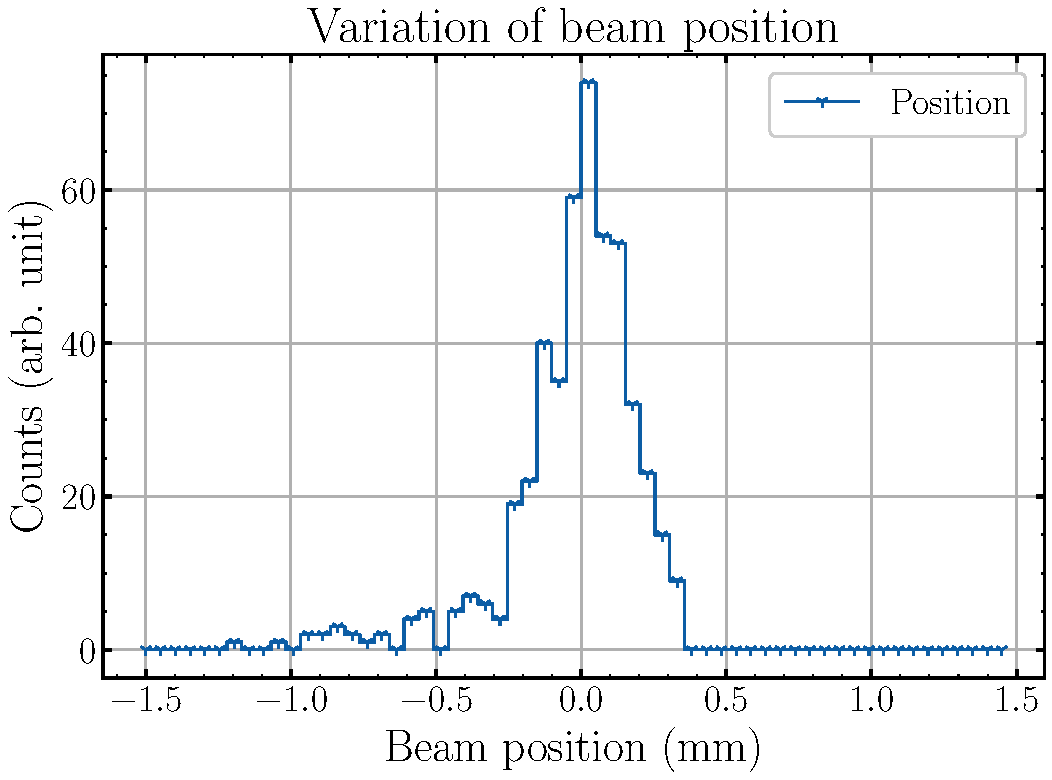
\includegraphics[width=1\textwidth]{04_Test/fig/fig000_hist_variation_a}
    \end{column}
    \begin{column}{0.45\textwidth}
      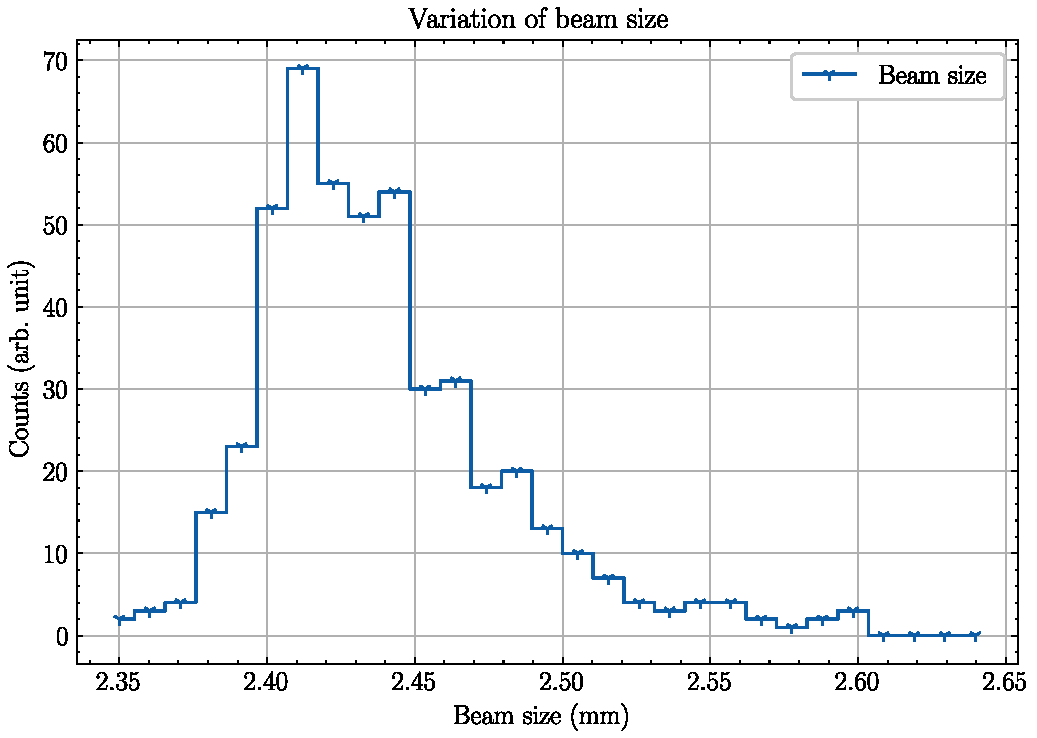
\includegraphics[width=1\textwidth]{04_Test/fig/fig000_hist_variation_b}
      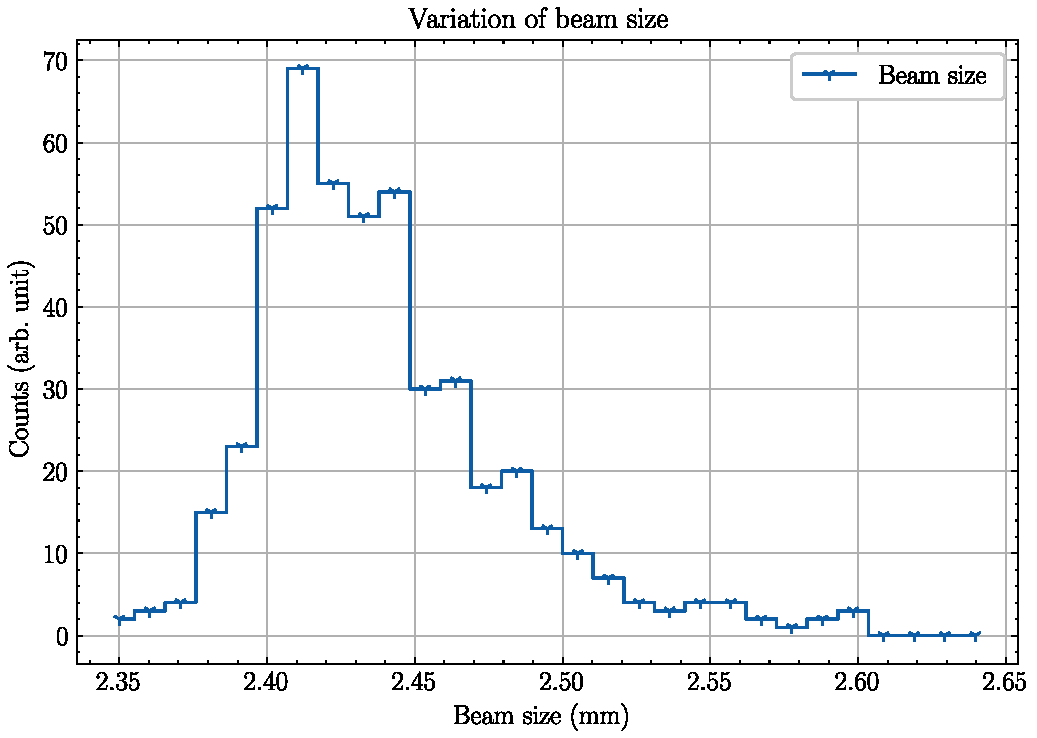
\includegraphics[width=1\textwidth]{04_Test/fig/fig000_hist_variation_b}
    \end{column}
  \end{columns}
  \begin{alertblock}{}
    Unfortunately there is no profile monitor on IPHI.
  \end{alertblock}
\end{frame}

\begin{frame}
  \frametitle{Comparison with IHPI diagnostic}
  \begin{alertblock}{}
    Unfortunately there is no profile monitor on IPHI.
  \end{alertblock}
\end{frame}

\begin{frame}
  \frametitle{Limits}
  \begin{alertblock}{}

  \end{alertblock}
\end{frame}

\begin{frame}
  \frametitle{Limits}
  \begin{alertblock}{}
    Checking the field wrt to the size variation
  \end{alertblock}
\end{frame}

\begin{frame}
  \frametitle{Limits}
  \begin{columns}[T]
    \begin{column}{0.45\textwidth}

    \end{column}
    \begin{column}{0.45\textwidth}
      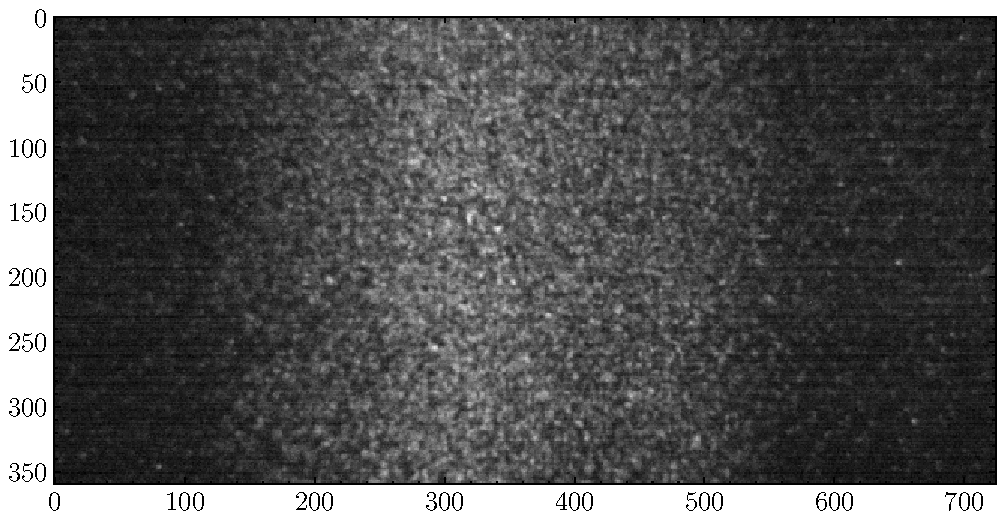
\includegraphics[width=1\textwidth]{04_Test/fig/fig000_limits_IPHI_a}
      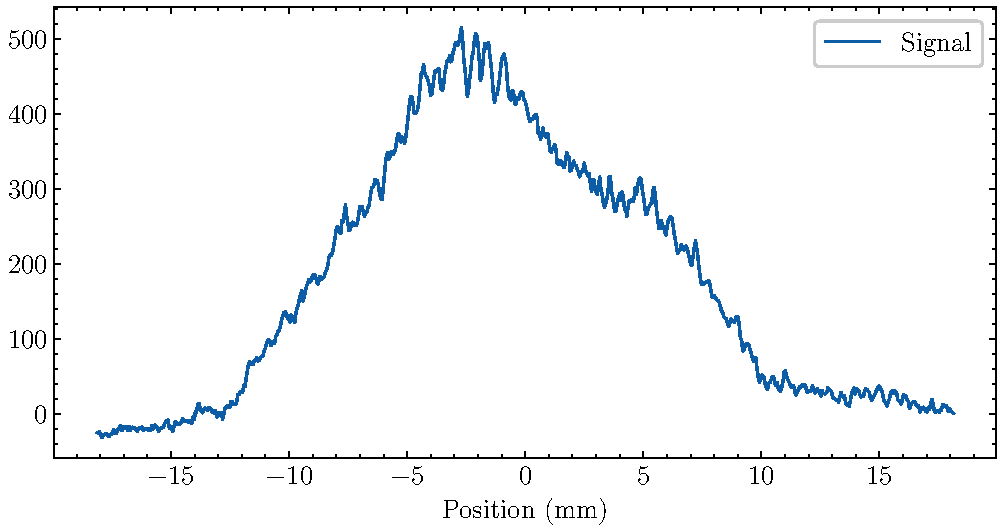
\includegraphics[width=1\textwidth]{04_Test/fig/fig000_limits_IPHI_b}
    \end{column}
  \end{columns}
  \begin{alertblock}{}
    Even a single stage MCP seems to be sufficient to detect profile.
  \end{alertblock}
\end{frame}